\section* {3.4}

\subsection{Постановка задачи}
Вычислить первую и вторую производную от таблично заданной функции $y_i=f(x_i), i=0,1,2,3,4$  в точке $x=X_i$.   

{\bfseries Вариант:} 10
$X^*=1.0$

\begin{figure}[h!]
\centering
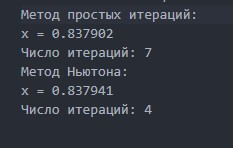
\includegraphics[width=15cm, height=2cm]{img1}
\caption{Условия}
\end{figure}
%\pagebreak

\subsection{Результаты работы}
\begin{figure}[h!]
\centering
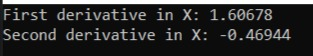
\includegraphics[width=10cm, height=2cm]{img}
\caption{Вывод программы в консоли}
\end{figure}
\pagebreak
% \vfill


\subsection{Исходный код}
% \lstinputlisting[language=C++]{matrix.cpp}
% \begin{lstlisting}
\lstinputlisting{include/3_4.cpp}
% \end{lstlisting}
% \lstinputlisting{matrix.cpp}
% {../../include/matrix.cpp}
% \pagebreak
% \lstinputlisting[title=\texttt{parabolic\_pde.hpp}]{../../include/partial_differential/parabolic_pde.hpp}
% \pagebreak
% 